% !TEX root = webmatematik.tex

\section{Konfidensintervaller}
Hvis vi ønsker at bestemme middelværdien for højden af alle gymnasieelever i
Danmark, kan vi fx udvælge en 1.g.\ klasse i Københavner området og beregne
middelværdien for de studerendes højde i denne klasse.

Den beregnede middelværdi er så et estimat for middelværdien for højden for alle
gymanisie elever i Danmark. Hvis vi nu vælger en anden klasse og igen beregner
middelværdien, så får vi et andet estimat for middelværdien.

Dette estimat ligger sikkert tæt på den første beregnede middelværdi uden at være
identisk med denne. Vi kalder det at udvælge en gymnasieklasse for tage en stikprøve
ud af den samlede \textbf{population} bestående af samtlige gymnasieelever i Danmark.

Stikprøvens middelværdi kaldes også for et punktestimat for populations
middelværdi. Men hvis to forskellige stikprøver giver to forskellige estimater for
middelværdien, hvordan kan vi så stole på estimatet. Hvad nu hvis vi i stedet for
bare et enkelt punktestimat kunne bestemme et interval, som med stor sandsynlighed
indeholder den rigtige ukendte middelværdi for hele populatioen.

Et sådan interval kaldes også for et konfidensinterval. Et konfidensinterval er
kendetegnet ved et niveau \(1 - \alpha\) og en typisk værdi for \(\alpha\) er \(5\),
hvor man så taler om et \(1-\alpha = 95\%\) konfidensinterval.

\subsection{Formel}
Hvis vi antager, at gymnasieelevers højde er normalfordelt med ukendt middelværdi
\(\mu\) og en kendt spredning på \(\sigma\), så er formlen for et
\(95\%\)-konfidens\-interval

\begin{equation}
  95\%\mbox{-konfidensinterval} = \Big[\bar{x} - 1,96⋅\frac{\sigma}{\sqrt{n}};
  \bar{x} +1,96⋅\frac{\sigma}{\sqrt{n}} \Big],
\end{equation}
hvor
\begin{itemize}
  \item \(\bar{x}\) er stikprøvens middelværdi og
  \item \(n\) er stikprøvens størrelse.
\end{itemize}
Vi vender tilbage til konstanten \(1,96\).

\subsection{Eksempel}
Hvis vi antager at gymnasieelevers højde er normalfordelt med ukendt middelværdi
\(\mu\) og standard afgivelse på \(\sigma=10\mbox{cm}\), og vi har følgende
stikprøve på 27 elevers højde (målt i cm)

\begin{align*}
  &175, 161, 177, 173, 179, 174, 173, 184, 184, 170, 169, 175, 175, 186, \\
  &169, 169, 176, 166, 181, 175, 179, 179, 183, 166, 179, 160, 170
\end{align*}

så kan vi beregne stikprøvens middelsværdi til 174,33 og derfor er \(95\%\)-kon\-fi\-dens\-in\-ter\-val\-let bestemt ved
\begin{align*}
  \Big[174,33 - 1,96 \frac{10}{\sqrt{27}}; 174,33 + 1,96 \frac{10}{\sqrt{27}} \Big]
  &=\Big[174,33 - 3,77 ; 174,33 + 3,77 \Big] \\&= \Big[ 170,56; 178,10\Big]
\end{align*}

\subsection{Konstanten 1,96}
Hvor kom konstanten 1,96 fra som indgik i formlen for
\(95\%\)-konfidens\-in\-ter\-val\-let? Hvis vi kigger for fordelingsfunktionen for
en normalfordeling med middelværdi 0 og varians 1, så er det samlede areal under
kurven 1. Hvis vi derfor er interesseret i at finde det område under grafen, som
dækker 95\% af arealet, skal vi altså fjerne 2,5\% af arealet i begge ender.

\begin{center}
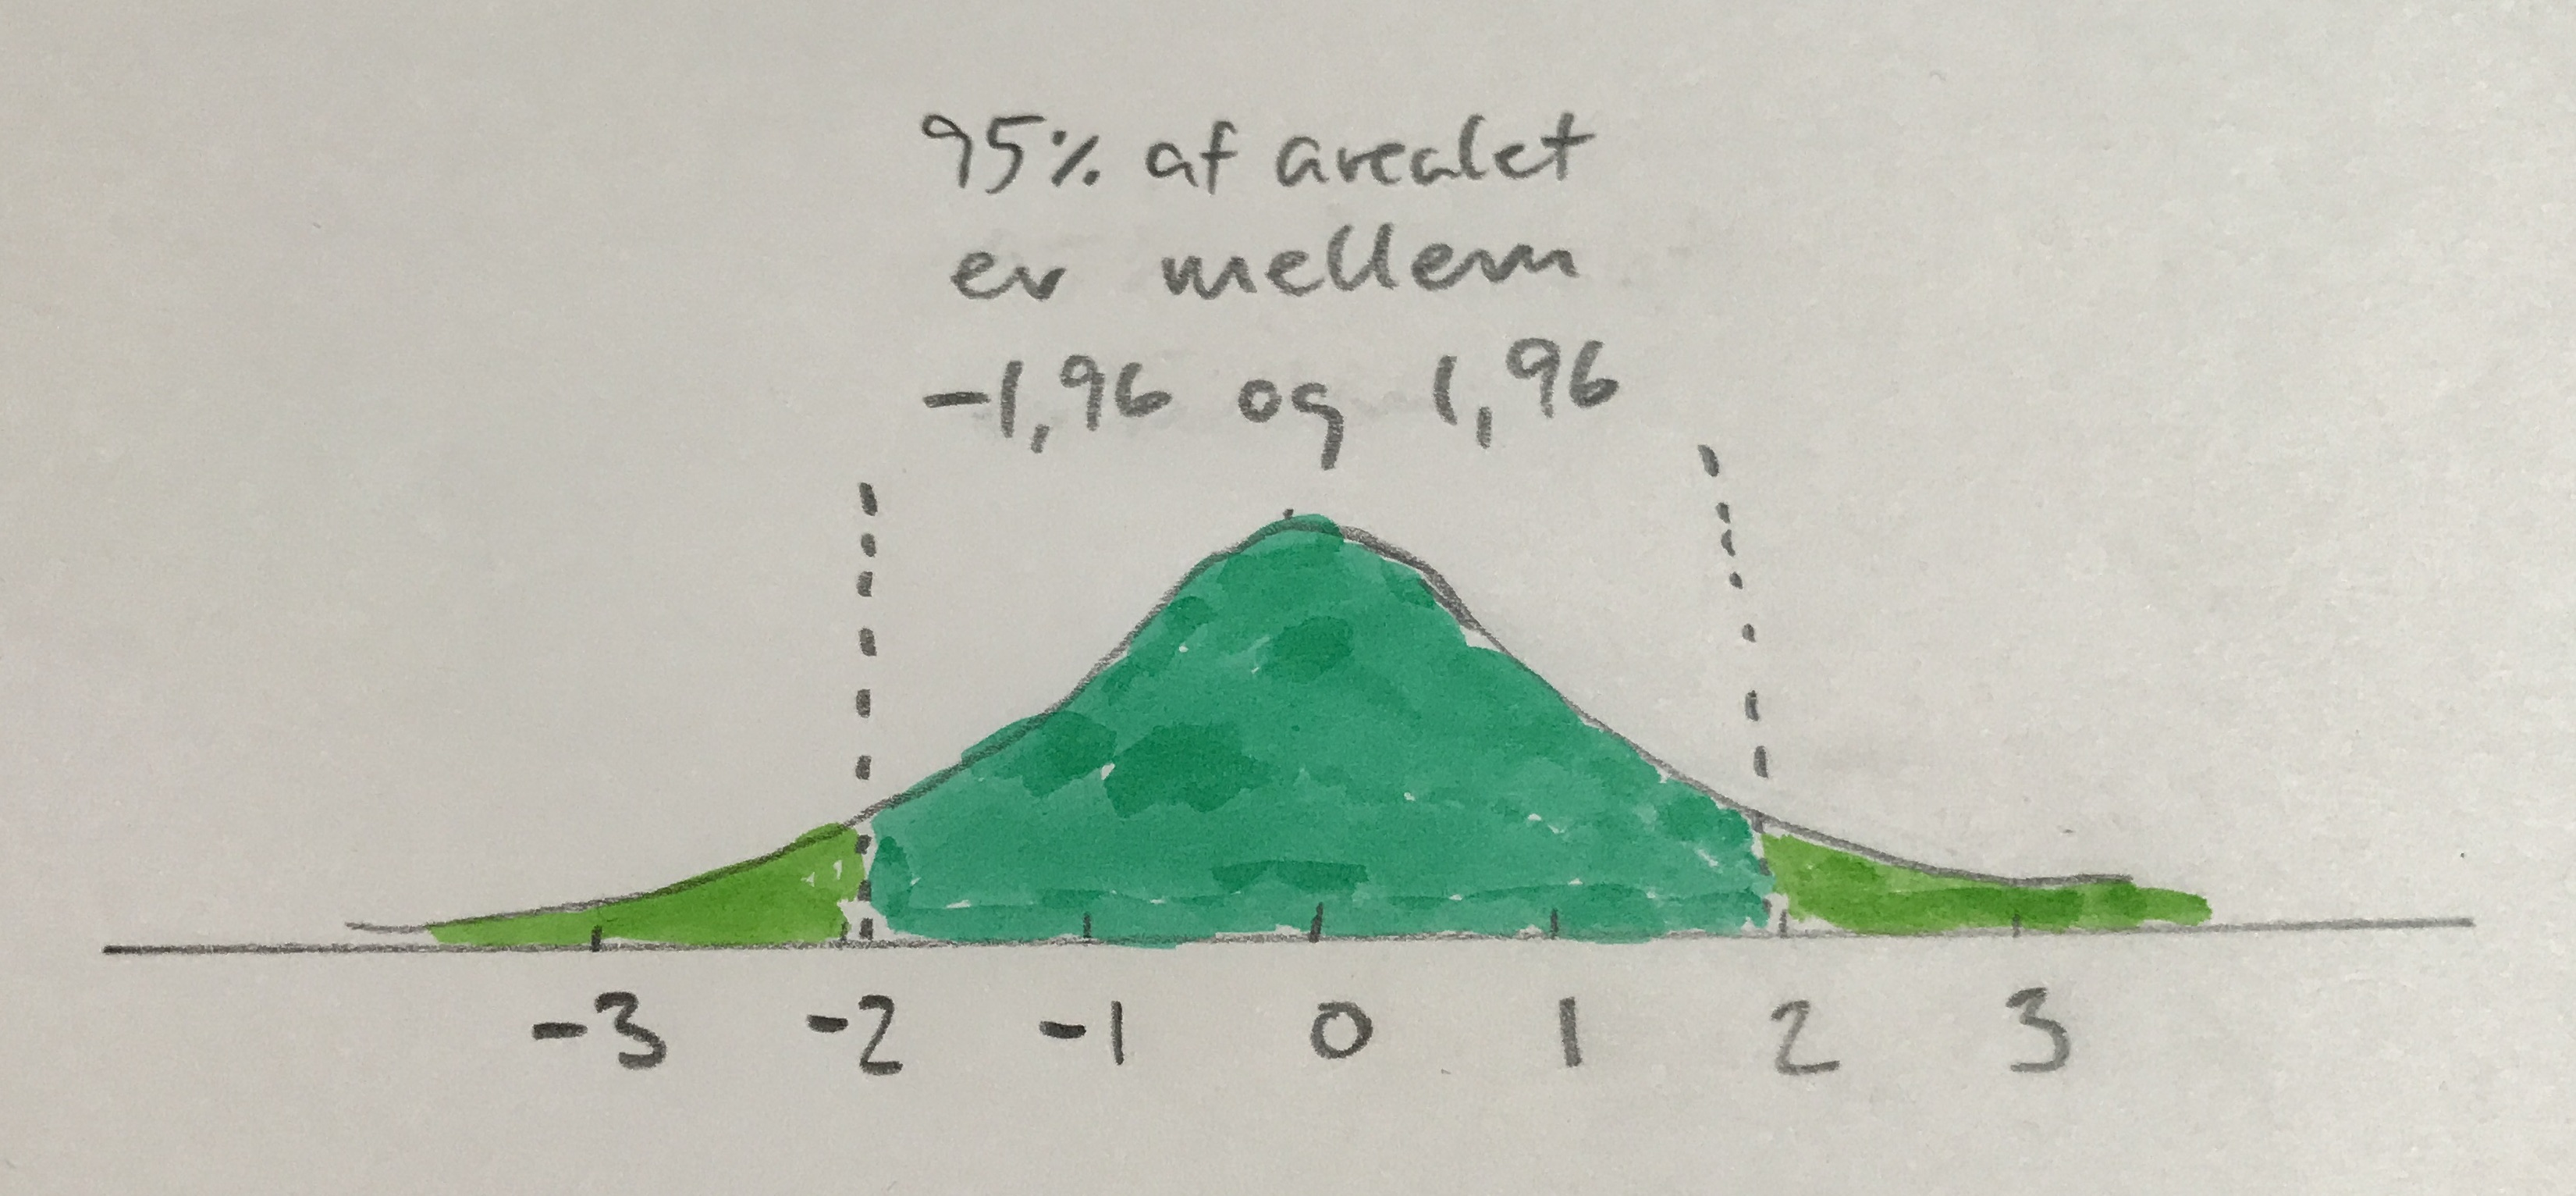
\includegraphics[height=6cm]{normalfordeling.JPG}
\end{center}

De \(\plusminus 1,96\) svarer præcis til det område under kurven som giver en areal
på 95\%. Andre ofte anvendte konfidensintervaller er angivet i denne tabel.

\begin{table}[]
\centering
\begin{tabular}{@{}|l|r|@{}}
\toprule
Konfidensniveau & \multicolumn{1}{l|}{konstant} \\ \midrule
68\%            & 1                             \\ \midrule
90\%            & 1,645                         \\ \midrule
95\%            & 1,96                          \\ \midrule
99\%            & 2,58                          \\ \bottomrule
\end{tabular}
\end{table}

Hvis man skal regne fx et 90\% konfidensinterval skal konstanten 1,96 erstattes med
1,645.

For man brug for at bestemme andre konstanter kan man bruge Microsodt Office Excel
til at udregne disse. Skal man bestemme et 92\% konfidensinterval kan man finde
konstanten med funktionen NORMSINV i Excel. Her skal man så udregne
\(1-\alpha = 0,92\) så \(\alpha = 0,08\) og herefter indsætter man

\begin{equation}
  \mbox{NORMSINV} \Big( 1-\frac{0,08}{2} \Big) = 1,75
\end{equation}

Matlab fra MathWorks har tilsvarende funktionalitet. Her bruger man funktionen
norminv
\begin{equation}
  \mbox{norminv}\big([0.04; 0.96], 0, 1\big),
\end{equation}
hvor 0 angiver middelværdien og 1 variansen.

\subsection{Konfidensinterval for binominalfordelinger}
Ved en rundspørge på et gymnasie har 62 af 1.g. elever sagt, at de var tilfredse
med introduktionsforløbet. 29 elever svarede, at de ikke var tilfredse.

Hvordan bestemmer man et \(95\%\)-konfidens\-interval for andelen af tilfredse
elever? Hvis \(X\) er antallet af elever som er tilfredse med introduktionsforløbet
ud af en stikprøve på 62+29=91, så er X binominalfordelt
\(X \sim b\big(n=91,p \big)\)

Vi har her en fast med ukendt sandsynlighed for at der bliver succes. Denne
paramater kaldes sandsynlighedsparameteren og betegnes \(p\).
Sandsynlighedsparameteren kan estimeres til \(\widehat{p}\)

\begin{equation}
  \widehat{p} = \frac{62}{91} = 0,68
\end{equation}

\subsection{Formel}
Formlen for et  \(95\%\)-konfidens\-interval i binominalfordelingen er
\begin{equation}
  \Bigg[ \widehat{p} - 1,96 \sqrt{\frac{\widehat{p}\big(1-\widehat{p}\big)}{n}} ;
  \widehat{p} + 1,96 \sqrt{\frac{\widehat{p}\big(1-\widehat{p}\big)}{n}} \Bigg]
\end{equation}

Indsætter vi i denne formel findes konfidensintervallet
\begin{equation}
  \Bigg[ 0,68 - 1,96 \sqrt{\frac{0,68\big(1-0,68\big)}{n}} ;
  0,68 + 1,96 \sqrt{\frac{0,68\big(1-0,68\big)}{n}} \Bigg] =
  \Big[0,58  ; 0,78  \Big]
\end{equation}
Altså vil tilfredsheden med introforløbet med 95\% sikkerhed være mellem 58\% og
78\%.
